\subsection{$\mathbb{F}$ is $\mathbb{R}$}

Turns out that there is a reason why it is called \textbf{\textit{Real}} Analysis. So far we have worked over a generic \textit{Complete Ordered Field} $\mathbb{F}$, that was also an \textit{Archimedean} following the expected properties. We have finally reached the point were we can state that \textbf{any} set that manages to follow all these properties is actually identical to the set of real numbers $\mathbb{R}$. In fact, $\mathbb{R}$ is the only set that accomplishes this.

Most Real Analysis courses don't go into proving this, but as I already mentioned in the first chapter, I want to cover all doubts and missing point existent during a course like this.

We will go through the initial proofs needed to understand the main one. At the beginning its possible that some of them look unecessary or trivial, but I don't want to assume that much. Better to be safe than sorry.

\subsubsection{Isomorphism}

Our starting point will be defining what it means to have \textquotedblleft equal fields".


\begin{definition}[Field homomorphism]
Let $F, F^\prime$ fields. A function $\phi: F \rightarrow F^\prime$ is a homomorphism between $F$ and $F^\prime$ iif. it preserves the defined operations in both fields:
\begin{align*}
\phi(x + y) &= \phi(x) + \phi(y), \forall x, y \in F\\
\phi(x . y) &= \phi(x) . \phi(y), \forall x, y \in F
\end{align*}
\end{definition}

\begin{definition}[Field isomorphism]
Let $F, F^\prime$ fields. A function $\phi: F \rightarrow F^\prime$ is a isomorphism iif. it is a homomorphism and also a bijection
\end{definition}

\begin{lemma}[Injectivity by order preservation]
Let $F, F^\prime$ fields, $\phi: F \rightarrow F^\prime$. If $\phi$ preserves order from $\mathbb{F}$:
$$x < y \Rightarrow \phi(x) < \phi(y), x, y \in F$$
Then $\phi$ is injective.
\end{lemma}

\begin{bookproof}
To prove injectivity, we need to show that for any two identical images of the function $\phi$, we get that their arguments were the same, guaranteeing the uniqueness of the image:

Let $x, y \in \mathbb{F}$ so that $$\phi(x) = \phi(y)$$

Using the tricotomy over $F$:

Case 1: $x < y$: $$\rightarrow \phi(x) < \phi(y) (\rightarrow\leftarrow)$$
Case 2: $y < x$: $$\rightarrow \phi(y) < \phi(x) (\rightarrow\leftarrow)$$

$$\Rightarrow x = y$$

Then, $\phi$ is injective.
\end{bookproof}


\begin{lemma}[Surjectivity by construction]
Let $F, F^\prime$ fields, $\phi: F \rightarrow F^\prime$. Define: $$\text{Im}_F := \{\phi(x), x \in F\}$$
Then, the bounded function $\phi^\prime: F \rightarrow \text{Im}_F$ is surjective
\end{lemma}

\begin{bookproof}
To prove surjectivity, we need to show that every element in $y \in \text{Im}_F$ has an $x \in F$ such that $\phi^\prime(x) = y$

Using the definition of our constructed set:
\begin{align*}
\forall y \in \text{Im}_F \Leftrightarrow y \in \{\phi(x), x \in F\}\\
\Rightarrow \exists x \in F / \forall y \in \text{Im}_F: y = \phi^\prime(x)\\
\end{align*}

Finally proving that for any image of $\phi^\prime \in \text{Im}_F$ we will have a preimage $x \in F$.

Then $\phi^\prime$ is surjective.
\end{bookproof}

On this first part, this surjectiveness by construction might be the bit that doesn't quite seem correct. Isn't it trivial to have surjectiveness if we grab the method $\phi$ and limit it to its image $\phi^\prime$?

The key here is that we defined the set of images $\text{Im}_F$ first, and \textit{then} proved the surjectiveness in it. The lemma confirms that the set we defined was \textit{just right}. Not so big to leave some elements unreached, and not too small to make undefined preimages at some spots.

\subsubsection{Sets construction}

Now, to make it reasonable for a complete ordered field $\mathbb{F}$ to be isomorphic to our known $\mathbb{R}$, we need to start shaping it using the parts that make it up. Think of $\mathbb{R}$ as the joint set of irrational and rational numbers, which contain the other types of number as well.

\begin{figure}[h]
\centering
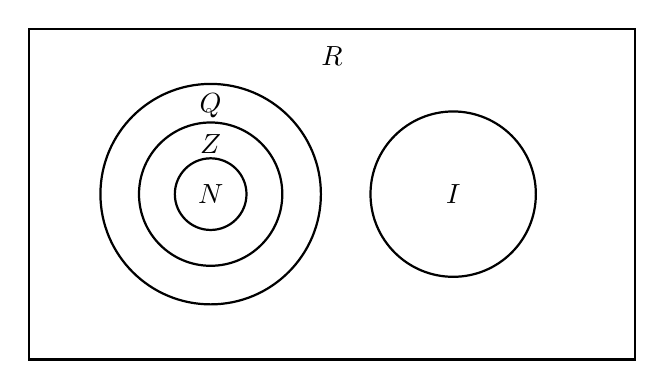
\begin{tikzpicture}[scale=0.7]
    % Real numbers rectangle (outermost)
    \draw[thick] (-5.5,-3) rectangle (5.5,3);
    \node at (0, 2.5) {$\mathbb{R}$};
    
    % Rational numbers circle (left side)
    \draw[thick] (-2.2,0) circle (2cm);
    \node at (-2.2, 1.6) {$\mathbb{Q}$};
    
    % Integers circle
    \draw[thick] (-2.2,0) circle (1.3cm);
    \node at (-2.2, 0.9) {$\mathbb{Z}$};
    
    % Natural numbers circle (innermost)
    \draw[thick] (-2.2,0) circle (0.65cm);
    \node at (-2.2, 0) {$\mathbb{N}$};
    
    % Irrational numbers circle (right side, disjoint)
    \draw[thick] (2.2,0) circle (1.5cm);
    \node at (2.2, 0) {$\mathbb{I}$};
    
\end{tikzpicture}
\captionsetup{width=0.8\textwidth}
\caption{\small{Hierarchy of number sets: Natural numbers ($\mathbb{N}$), Integers ($\mathbb{Z}$), Rationals ($\mathbb{Q}$), Irrationals ($\mathbb{I}$), and Real numbers ($\mathbb{R}$).}}
\label{fig:number_sets}
\end{figure}


From this idea, we need to build $\mathbb{N_F}$, $\mathbb{Z_F}$, $\mathbb{Q_F}$ and $\mathbb{I_F}$ to finall get this $\mathbb{F}$ we want to make some proofs on. This will all make sense in the last bit of the process, and I promise that the only tricky part will be to construct $\mathbb{I_F}$ from $\mathbb{Q_F}$, but we need to go step by step.


\begin{definition}[$\mathbb{N}_{\mathbb{F}}$ by induction]
Let $\mathbb{F}$ be \textit{the} complete ordered field. Using $1_\mathbb{F}$: multiplicative neutral of $\mathbb{F}$, we declare the following element contruction:

\begin{align*}
&1_\mathbb{F} := 1_\mathbb{F}\\
&2_\mathbb{F} := 1_\mathbb{F} + 1_\mathbb{F}\\
&3_\mathbb{F} := 1_\mathbb{F} + 1_\mathbb{F} + 1_\mathbb{F}\\
\vdots\\
&n_\mathbb{F} := \sum_{1}^{n}{1_F}
\end{align*}

Finally, we define the set:
$$\mathbb{N_F} := \{1_\mathbb{F}, 2_\mathbb{F}, 3_\mathbb{F}, \dots\} = \{n_\mathbb{F}: n \in \mathbb{N} \}$$
\end{definition}

\begin{definition}[$\mathbb{Z}_\mathbb{F}$ by extension]
Within field $\mathbb{F}$, let the following:
\begin{enumerate}
\item $0_\mathbb{F}$: Additive identity
\item $-x$: Additive inverse
\end{enumerate}

We define the set:
$$\mathbb{Z_F} = \{0_\mathbb{F}\} \cup \mathbb{N_F} \cup \{-x_\mathbb{F}, \forall n_\mathbb{F} \in N_\mathbb{F}\}$$
\end{definition}

\begin{definition}[$\mathbb{Q}_\mathbb{F}$ by operation]
Within field $\mathbb{F}$, we define the set:
$$\mathbb{Q_F} := \{\frac{a}{b}: a \in \mathbb{Z_F}, b \in \mathbb{N_F}\}$$
\end{definition}

Starting similarly to \cref{th:archimedean} (Archimedean property) we use the inductive approach to reach $\mathbb{N_F}$. Fancy but not complicated at all. Later, we just extend integers in $\mathbb{F}$ to build by $\mathbb{Z_F}$. Notice how we only used existent elements from $\mathbb{F}$ computed using the field's operations and nothing else.
